%%%%%%%%%%%%%%%%%%%%%%%%%%%%%%%%%%%%%%%%%
% Short Sectioned Assignment LaTeX Template Version 1.0 (5/5/12)
% This template has been downloaded from: http://www.LaTeXTemplates.com
% Original author:  Frits Wenneker (http://www.howtotex.com)
% License: CC BY-NC-SA 3.0 (http://creativecommons.org/licenses/by-nc-sa/3.0/)
%%%%%%%%%%%%%%%%%%%%%%%%%%%%%%%%%%%%%%%%%

%----------------------------------------------------------------------------------------
%	PACKAGES AND OTHER DOCUMENT CONFIGURATIONS
%----------------------------------------------------------------------------------------

\documentclass[paper=a4, fontsize=11pt]{scrartcl} % A4 paper and 11pt font size

% ---- Entrada y salida de texto -----

\usepackage[T1]{fontenc} % Use 8-bit encoding that has 256 glyphs
\usepackage[utf8]{inputenc}
%\usepackage{fourier} % Use the Adobe Utopia font for the document - comment this line to return to the LaTeX default

% ---- Idioma --------

\usepackage[spanish, es-tabla]{babel} % Selecciona el español para palabras introducidas automáticamente, p.ej. "septiembre" en la fecha y especifica que se use la palabra Tabla en vez de Cuadro

% ---- Otros paquetes ----

\usepackage{amsmath,amsfonts,amsthm} % Math packages
%\usepackage{graphics,graphicx, floatrow} %para incluir imágenes y notas en las imágenes
\usepackage{graphics,graphicx, float} %para incluir imágenes y colocarlas

% Para hacer tablas comlejas
%\usepackage{multirow}
%\usepackage{threeparttable}

%\usepackage{sectsty} % Allows customizing section commands
%\allsectionsfont{\centering \normalfont\scshape} % Make all sections centered, the default font and small caps

\usepackage{fancyhdr} % Custom headers and footers
\usepackage{url}
\usepackage{hyperref}
\pagestyle{fancyplain} % Makes all pages in the document conform to the custom headers and footers
\fancyhead{} % No page header - if you want one, create it in the same way as the footers below
\fancyfoot[L]{} % Empty left footer
\fancyfoot[C]{} % Empty center footer
\fancyfoot[R]{\thepage} % Page numbering for right footer
\renewcommand{\headrulewidth}{0pt} % Remove header underlines
\renewcommand{\footrulewidth}{0pt} % Remove footer underlines
\setlength{\headheight}{13.6pt} % Customize the height of the header

\numberwithin{equation}{section} % Number equations within sections (i.e. 1.1, 1.2, 2.1, 2.2 instead of 1, 2, 3, 4)
\numberwithin{figure}{section} % Number figures within sections (i.e. 1.1, 1.2, 2.1, 2.2 instead of 1, 2, 3, 4)
\numberwithin{table}{section} % Number tables within sections (i.e. 1.1, 1.2, 2.1, 2.2 instead of 1, 2, 3, 4)

\setlength\parindent{0pt} % Removes all indentation from paragraphs - comment this line for an assignment with lots of text

\newcommand{\horrule}[1]{\rule{\linewidth}{#1}} % Create horizontal rule command with 1 argument of height

\usepackage{booktabs}




%----------------------------------------------------------------------------------------
%	TÍTULO Y DATOS DEL ALUMNO
%----------------------------------------------------------------------------------------

\title{	
\normalfont \normalsize 
\textsc{{\bf Aprendizaje Automático (2014-2015)} \\ Grado en Ingeniería Informática \\ Universidad de Granada} \\ [25pt] % Your university, school and/or department name(s)
\horrule{0.5pt} \\[0.4cm] % Thin top horizontal rule
\huge Práctica 1 \\ % The assignment title
\horrule{2pt} \\[0.5cm] % Thick bottom horizontal rule
}

\author{Ignacio Martín Requena} % Nombre y apellidos

\date{\normalsize\today} % Incluye la fecha actual

%----------------------------------------------------------------------------------------
% DOCUMENTO
%----------------------------------------------------------------------------------------
\usepackage{graphicx}
\usepackage{listings}
\usepackage{color}
\definecolor{gray97}{gray}{.97}
\definecolor{gray75}{gray}{.75}
\definecolor{gray45}{gray}{.45}
 

\lstset{ frame=Ltb,
     framerule=0pt,
     aboveskip=0.5cm,
     framextopmargin=3pt,
     framexbottommargin=3pt,
     framexleftmargin=0.4cm,
     framesep=0pt,
     rulesep=.4pt,
     backgroundcolor=\color{gray97},
     rulesepcolor=\color{black},
     %
     stringstyle=\ttfamily,
     showstringspaces = false,
     basicstyle=\small\ttfamily,
     commentstyle=\color{gray45},
     keywordstyle=\bfseries,
     %
     numbers=left,
     numbersep=15pt,
     numberstyle=\tiny,
     numberfirstline = false,
     breaklines=true,
   }
 


\lstdefinestyle{consola}
   {basicstyle=\scriptsize\bf\ttfamily,
    backgroundcolor=\color{gray75},
   }
 
\lstdefinestyle{C}
   {language=C,
   }



\begin{document}

\maketitle % Muestra el Título

\newpage %inserta un salto de página

\tableofcontents % para generar el índice de contenidos

\listoffigures

%\listoftables

\newpage



%----------------------------------------------------------------------------------------
%	Cuestion 1
%----------------------------------------------------------------------------------------

\section{Cuestionario}

\subsection{Decir cuáles de los siguientes casos son un problema de regresión o de clasificación e indicar si estaremos más interesado en inferencia o en predicción. Identificar también los valores de n ( tamaño muestra) y p ( número de predictores):}


\subsubsection{Recopilamos un conjunto de datos de las 500 empresas españolas más grandes. Por cada compañía recogemos: beneficio anual, número de empleados, tipo de industria y sueldo del director. Estamos interesado en comprender que factores afectan al sueldo del director.}

Este es un problema de regresión y predicción, dado que lo que nos interesa no es predecir de que tipo es un determinado dato, si no estimar cual es el sueldo. El tamaño de la muestra es 500 y el número de predictores es 4.


\subsubsection{Estamos considerando lanzar un nuevo producto y deseamos conocer si será un éxito o un fracaso. Para ello recogemos datos de 20 productos semejantes ya existentes en el mercado. Para cada producto medimos: a) si fue un éxito o un fracaso; b) precio del producto; c) presupuesto de marketing; d) precio de oferta inicial y otras diez variables más}
Es un problema de clasificación en el que nos interesa hacer inferencia sobre el conjunto de datos. El tamaño de la muestra es 20 y poseemos 13 predictores. 

\subsubsection{Estamos interesados en predecir el \% de variación del euro respecto de los porcentajes de variación semanales de los mercados europeos. Para ello recogemos datos semanales de todo el 2012. En cada semana medimos el \% de cambio del euro, el \% de cambio de la bolsa Alemana, el \% de cambio de la Bolsa Inglesa y el \% de cambio de la bolsa Francesa.}
Es un problema de regresión en el que nos interesa hacer una predicción a partir de los datos obtenidos. El tamaño de la muestra es 52 (semanas que tiene un año) y el número de predictores es 4.

%----------------------------------------------------------------------------------------
%	Cuestion 2
%----------------------------------------------------------------------------------------

\subsection{Identificar dos aplicaciones empresariales (no comentadas en clase) en las que considere que las técnicas de Aprendizaje Automático serán útiles. Describir brevemente cada una de ellas, el interés de la misma y el problema que se resuelve. Identificar algunas de las variables que considere más importantes al problema. Describir un caso en que regresión será la técnica a aplicar (decir además si el problema es más de inferencia o de predicción) y otro de clasificación.}

\begin{itemize}

\item \textbf{Predecir el conjunto de las especies de aves presentes en una grabación de audio, recogidos en condiciones de campo }\footnote{\url{http://www.kaggle.com/c/mlsp-2013-birds}}:

Se trata de, a partir de un conjunto de grabaciones recogidas en un medio natural, ser capaz de construir un sistema que nos diga que aves son las que están piando en ese lugar. Esto es posible gracias al monitoreo acústico. Con esto podríamos, por ejemplo, conocer más a cerca de las migraciones de las aves, de sus comportamientos y hacer predicciones sobre cuando una población de un tipo determinado de ave se está viendo mermada.

Se trata de un problema de clasificación. Las variable mas importante es la frecuencia de sonidos que se recogen en la grabación, dado que a partir de ella determinaremos la especie de ave en concreto.

\item \textbf{Identificar a las personas que tienen un alto grado de psicopatía en función del uso de Twitter}\footnote{\url{http://www.kaggle.com/c/twitter-psychopathy-prediction}}:

El objetivo de este proyecto predecir el grado de psicpatía de un individuo a partir del lenguaje y lo expresado en su red social de twitter. Para esto se ofrece una base de datos con 377 variables derivadas de información de gente anónima y una puntuación de psicopatía estan basadas en una lista de verificación desarrillada por la Universidad de Columbia. A demás también se intenta examinar que se puede predecir a partir de la información generada en redes sociales y como esta puede ser utilizada.

Se trata de un problema de regresión, en el que nos interesa obtener un modelo que nos ayude a predecir el coeficiente de psicopatologia de un determinado usuario. Tenemos 377 predictores.

\end{itemize}
\newpage
%----------------------------------------------------------------------------------------
%	Cuestion 3
%----------------------------------------------------------------------------------------

\subsection{Describir las diferencias entre las aproximaciones supervisadas paramétricas y las no-paramétricas. ¿Cuáles son las ventajas de la aproximación paramétrica en regresión y en clasificación? ¿Cuáles las desventajas? Justificar la respuesta.}

En la aproximación paramétrica se supone que el conocimiento de la estructura estadística de las clases y se modelaban mediante funciones de densidad de probabilidad conocidas, por lo que el aprendizaje se basa en la estimación de los parámetros que determinan las funciones de densidad de probabilidad de las clases.

Por contra, en las aproximaciones no-maramétricas no se conoce este conocimiento a priori. Esta aproximación engloba muchas y muy diferentes técnicas como la estimación del valor de la función de densidad o lo que se conoce como aprendizaje adaptativo. \footnote{\url{http://iie.fing.edu.uy/ense/asign/recpat/material/tema3_00-01/node2.html}}

%----------------------------------------------------------------------------------------
%	Cuestion 4
%----------------------------------------------------------------------------------------

\subsection{Si tenemos un problema de clasificación con dos variables predictoras y nos muestran las fronteras de decisión de un clasificador kNN para distintos valores de k ¿Cómo podemos saber si la frontera de decisión comienza a estar sobre-ajustada? Justificar la respuesta.}

La frontera de decisión empezará a estar sobreajustada cuando los valores de k sean muy pequeños. Esto ocurre porque la frontera de decisión se ajusta a partir del valor de k y para valores pequeños, por ejemplo k=1, como solo cogemos el dato mas cercano con respecto al de entrada para determinar como clasificarlo, la frontera de decisión se pegará mucho a los datos de la muestra en vez de al modelo real.


\newpage
%----------------------------------------------------------------------------------------
%	Cuestion 5
%----------------------------------------------------------------------------------------

\subsection{Suponga que tenemos un conjunto de datos con 5 variables predictoras, X1, X2, X3, X4, X5, de las cuales X1 y X2 son cuantitativas, X3 es cualitativa con dos valores (0=hombre, 1=mujer), X4 representa la interacción entre X1 y X2 , y X5 representa la interacción entre X1 , y X3 . La variable de salida representa el valor del salario de hombres y mujeres. Hemos ajustado un modelo por mínimo cuadrados y se han obtenido los siguientes coeficientes B0 = 50, B1 = 20, B2 = 0.07, B3 = 35, B4 = 0.01, B5 = -10.}

\subsubsection{¿Cuáles de las siguientes contestaciones es correcta y por qué?}

\begin{itemize}

\item Para valores fijos de X1 y X2 los hombres ganan más en promedio que las mujeres.

\textbf{FALSO}. Para valores fijos de X1 y X1, los hombres no tendrán el sumando de 35*X3, por lo que su salario será menor. 

\item Para valores fijos de X1 y X2 las mujeres ganan más en promedio que los hombres.

\textbf{VERDADERO}. En este caso, como X3 = 1, el hecho de ser mujer haría que nuestra variable de salida fuera mayor que si fuera un hombre X3 = 0.


\item Para valores fijos de X1 y X2 los hombres ganan más en promedio que las mujeres con tal que X1 sea suficientemente grande.

\textbf{VERDADERO}. Esto es debido a que X4 representa la interacción entre X1 y X2 y, por tanto, para valores grandes de X1 el valor de X5 también sería grande y si fuera una mujer, al ser X3 = 1 restará lo suficiente como para penalizar el hecho de ser mujer y beneficiar el de ser hombre.

\end{itemize}

\subsubsection{Predecir el salario de una mujer con X1 = 4.0 y X2 =110}

Simplemente tenemos que substituir en la recta los valores proporcionados:\\

\begin{center}50+20*4+0.07*110+35+0.01*4*110-10*4*1 = \textbf{137.1}\end{center}
\newpage
\subsubsection{Dado que el coeficiente de X4 es pequeño existe poca evidencia de un efecto de
interacción entre X1 y X2, ¿ Verdadero o Falso? Justificar la respuesta}

\textbf{FALSO}. Lo que esto quiere decir es que la repercusión de la interacción entre X1 y X2 en el modelo es poca. Para saber si existe mucha o poca evidencia de un efecto de interacción tendríamos que mirar el valor Prob>|t|

%----------------------------------------------------------------------------------------
%	Cuestion 6
%----------------------------------------------------------------------------------------

\subsection{Tenemos un conjunto de datos de 100 observaciones con una única variable predictor y una respuesta cuantitativa. Ajustamos a dichos datos un modelo de regresión lineal Y = B0 + B1 X + e y un modelo de regresión cúbico Y = B0 + B1 X + B2 X2 + B3 X3 + e}


\subsubsection{Supongamos que la verdadera relación entre X e Y es lineal, es decir Y = B0 + B1 X + e . Considerar la suma de los residuos de los datos de entrenamiento (RSS) tanto para el modelo lineal como para el modelo cúbico. ¿Deberíamos esperar que en general un valor fuera menor que el otro, que fueran iguales, o no hay suficiente información para establecer una opinión por adelantado?}

Para el modelo de regresión lineal deberían haber un menor número de residuos de datos de entrenamiento ya que este se ajustará con más facilidad al comportamiento real de los datos, mientras que el modelo cúbico necesitará más RSS para representar la realidad.

\subsubsection{Contestar lo mismo del punto anterior pero considerando la sumas RSS de los datos de test.}

Para el modelo de regresión cúbico tendría un menor valor de RS,  ya que se sobreajustaría mas a los datos.

\subsubsection{Supongamos que la verdadera relación entre X e Y es no lineal, pero no conocemos como de lejos está de ser lineal. Consideremos las sumas RSS de entrenamiento para el modelo lineal y el cúbico ¿Deberíamos esperar que en general un valor fuera menor que el otro, que fueran iguales, o no hay suficiente información para establecer nada por adelantado? Justificar la contestación.}

Cabría esperar que el modelo de regresión lineal tuviera un mayor valor de RSS que el cúbico, ya que el cúbico tendría mas facilidad para adaptarse al modelo real.

\subsubsection{Contestar lo mismo del punto anterior pero considerando la sumas RSS de los datos de test.}

No habría manera de determinalo ya que no conocemos lo lejos que esta del modelo lineal y por tanto dependería de cada caso en concreto.

\newpage
\section{Ejercicios de implementacion}

%----------------------------------------------------------------------------------------
%	Cuestion 1
%----------------------------------------------------------------------------------------
\subsection{Usar la base de datos de Boston que es parte de la librería MASS en R:}

\subsubsection{Leer la descripción de la base de datos “help(Boston)”. Tratar de comprender el problema, identificar las variables del problema y hacer una valoración de la relevancia de las mismas para el estudio.}

La base de datos contiene información a cerca de datos obtenidos en suburbios de Boston. En concreto contiene las siguientes variables:

\begin{itemize}

\item \textbf{crim}: Representa la tasa de criminalidad per capita en la ciudad. En principio esta variable puede que tenga gran relevancia, dado que a partir de esta podremos predecir la tasa de criminalidad en un suburbio de Boston.

\item \textbf{zn}: Viviendas que poseen un suelo residencial dividido en zonas de mas de 25000 pies cuadrados. Puede que sea importante a la hora de estimar en que zonas las casas son mas grandes que en otras.

\item \textbf{indus}: Proporción de empresas por ciudad. Para estimar si la tasa de criminalidad o, por ejemplo, si en zonas con muchas empresas la concentración de oxido de nitrogeno aumenta.

\item \textbf{chas}: Indica si está cerca del río Charles. No creo que este predictor sea muy relevante.

\item \textbf{nox}: Concentración de oxido de nitrogeno. Quizá sea interesante para conocer donde hay mayor o menor contaminación.

\item \textbf{rm}: Media de habitaciones por casa. Quizá para conocer el nivel de ocupación en un determinado suburbio.

\item \textbf{age}: Proporcion de dueños de casas construidas a partir de 1940. Esta variable nos puede interesar para conocer si algún suceso ocurre en zonas desfavorecidas y antiguas.

\item \textbf{dis}: Media ponderada de las distancias a cinco centros de empleo de Boston.

\item \textbf{rad}: Índice de accesibilidad a las autovías.

\item \textbf{tax}: Impuestos que se pagan en un suburbio.

\item \textbf{ptratio}: Ratio de alumnos por profesor en una ciudad.

\item \textbf{black}: Proporción de personas negras en una ciudad.

\item \textbf{lstat}: Valor del estatus mas bajo de la población.

\item \textbf{medv}: Mediana del valor de las casas dividido entre \$1000s

\end{itemize}

\subsubsection{Realizar tres gráficos con las parejas de columnas que considere de más interés. Describir lo que has encontrado justificando la elección de las columnas estudiadas para el problema.}

\begin{itemize}

\item crim - black

Es posible que la criminalidad pueda verse influida por el color de la piel, dado que en ciudades como Boston esta gente por lo general se encuentra en riesgo de exclusión social y suelen carecer de infraestructuras y recursos.

\begin{figure}[H]
\centering
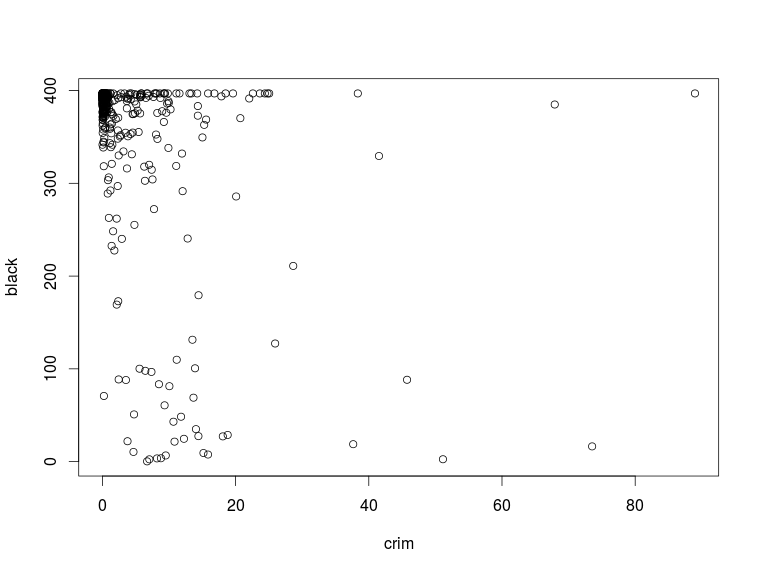
\includegraphics[scale=0.50]{cromblack.png}
\caption{crim vs black}
\label{}
\end{figure}

En la gráfica podemos ver que la mayoría de las muestras de criminalidad se han tomado en personas negras. Aun así el índce de criminalidad no es excesivamente alto en este grupo de gente y no podemos decir que la criminalidad esté relacionada con el color de piel.

\item age - tax

Otra posible relación sería la existente entre la antiguedad de una vivienda y el valor de la vivienda

\begin{figure}[H]
\centering
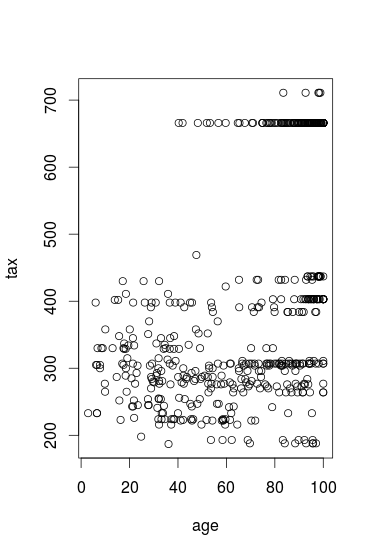
\includegraphics[scale=0.70]{agevstax.png}
\caption{age vs tax}
\label{}
\end{figure}

Contrariamente a lo que pensaba los datos de la gráfica están muy dispersos y no se observa ninguna dependencia entre ambas variables.

\item nox - indus

Sería interesante representar la cantidad de concenctración de oxido de nitrogeno frente a la proporción de empresas en una ciudad, dado que a primera vista puede ser que ambas variables estén relaccionadas

\begin{figure}[H]
\centering
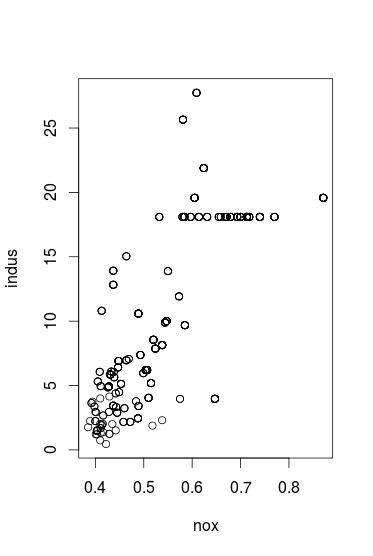
\includegraphics[scale=0.70]{noxvsindus.png}
\caption{nox vs indus}
\label{}
\end{figure}

Podemos intuir que a mayor nivel de oxido de nitrógeno es de esperar que la cantidad de industrias en la ciudad aumente.

\end{itemize}

\subsubsection{¿Existen predictores asociados con la tasa de crimen per capita? Si es así explicar la relación.}

Si, por ejemplo entre el crimen y elptratio. Solo hay que obvservar la gráfica que nos muestra R representando estas dos variables:


\begin{figure}[H]
\centering
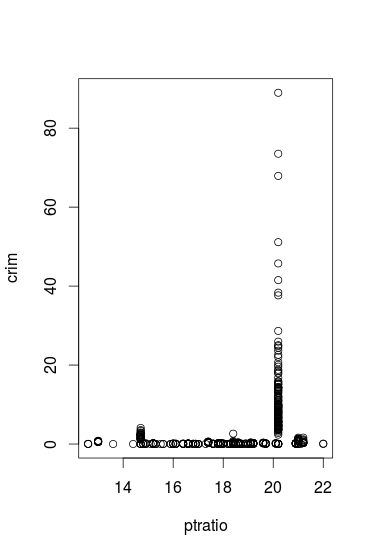
\includegraphics[scale=0.70]{crimvsptratio.png}
\caption{crim vs ptratio}
\label{}
\end{figure} 

Podemos ver como cuando el ptratio es de valor 20 la criminalidad sube de manera considerable.
\newpage
\subsubsection{Hay algún suburbio de Boston que parezca tener una alta tasa de: a) criminalidad, b) altos impuestos, c) alumnos-por-profesor. Comentar el rango de cada predictor.}

\begin{itemize}

\item a) Si, de hecho los valores más altos se encuentran en los suburbios que están rondando la fila 400, y el que mas valor posee ees el de la fila 381. El rango de criminalidad está entre 0 y 89.

\item b) Los suburbios en las filas que van desde la 489 a la  493 son los que poseen una mayor tasa de impuestos, con un valor de 711. El rango de impuestos va desde 188 a 711.

\item c) Hay un suburbio que posee la mayor tasa de alumnos por profesor, aunque no es una tasa muy elevada con respecto al resto de subirbios. En concreto el 355 y el 356 con un indice de 22 alumnos por profesor. EL rango por tanto esta entre 12.6 y 22.


\end{itemize}

\subsubsection{¿Cuántos suburbios de este conjunto de datos bordea o cruza el rio Charles?}

Hay 35 suburbuos que lo bordean o lo cruzan.

\subsubsection{¿Cuál es la media de la tasa alumnos-profesor entre las ciudades de este conjunto de datos?}

La media de la tasa alumnos-profesor es de 18.45553.

\subsubsection{¿Qué suburbio de Boston tiene el valor mediano más bajo de propietarios viviendo en sus casas? ¿Cuáles son los valores de los otros predictores para este suburbio, y como se comparan estos valores con el rango global de los otros predictores? Comentar los resultados.}

El sburvio con valor mediano mas bajo es el 399 con un valor de 5. El resto de valores son:

\begin{figure}[H]
\centering
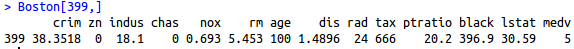
\includegraphics[scale=.70]{boston399.png}
\caption{Suburbio 399 Boston}
\label{}
\end{figure}

En este suburbio se ver como, por ejemplo, tiene unos altos índices de alumnos-profesor, de criminalidad (la media de indice de criminalidad es de 3,6), de ciudadanos negros y de tasas. Fijandonos solamente en el valor de los preictores podemos intuir que se trata de un suburbio con un nivel de conflictividad alto.

\subsubsection{¿Cuántos de los suburbios tienen en promedio más de siete habitaciones por vivienda? ¿más de ocho por vivienda? Haga algún comentario al caso cuyo promedio de habitaciones por vivienda sea mayor de ocho.}

\begin{itemize}

\item Viviendas con más de \textbf{siete} habitaciones por vivienda: 64

\item Viviendas con más de \textbf{ocho} habitaciones por vivienda: 13



\end{itemize}

\newpage
%----------------------------------------------------------------------------------------
%	Cuestion 2
%----------------------------------------------------------------------------------------

\subsection{Para la base de datos Boston}

\subsubsection{Predecir la ratio de crímenes per-capita usando las otras variables en la base de datos Boston}

\begin{itemize}

\item Para cada predictor ajustar un modelo de regresión lineal simple con la variable respuesta. Describir los resultados

Ajustando un modelo de regresión lineal para cada predictor y observando los valores de la pendiente y el corte con el eje Y que R nos muestra podemos ver como, por ejemplo, el modelo que hay entre los predictores crim y chas nos hace ver que es un modelo con poco crecimiento y con pendiente negativa, por lo que intuyo que no habrá mucha relación, o si la hay, será poco significativa. También podemos ver que el modelo que obtenemos al ajustar crim y nos también tiene unos coeficientes algo "raros" en cuanto a que se observa un valor muy alto de pendiente (31.25) en comparación con e resto de modelos. 

\item ¿En qué modelos existe una asociación estadísticamente significativa entre predictor y respuesta?

Observando el p-valor y el Pr(>|t|) podemos ver como por ejemplo el error que cometemos al coger la variable rm es insignificante, al igual que ocurre con rad.

\item Crear algún gráfico que muestre los ajustes y que valide las respuestas.

\begin{figure}[H]
\centering
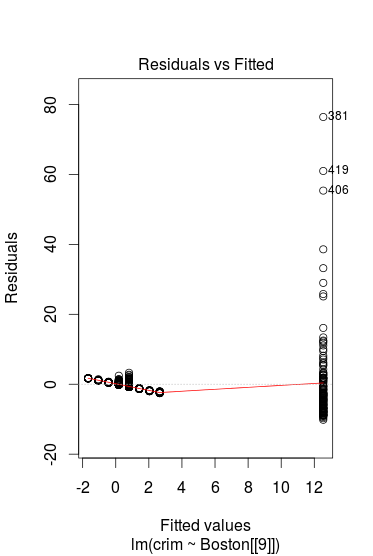
\includegraphics[scale=.60]{regcrimrad.png}
\caption{Regresión crim vs rad}
\label{}
\end{figure}

\begin{figure}[H]
\centering
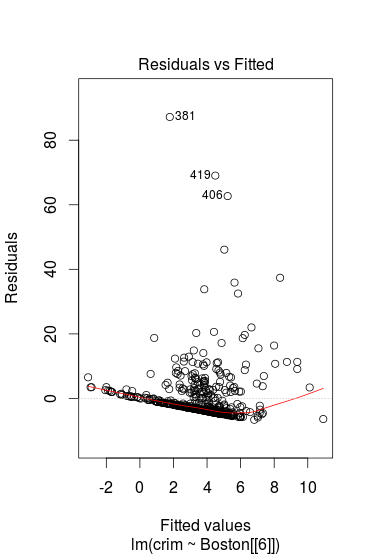
\includegraphics[scale=.60]{regcrimrm.png}
\caption{Regresión crim rm}
\label{}
\end{figure}

\end{itemize}


\subsubsection{Ajustar un modelo de regresión múltiple usando todos los predictores.}

\begin{itemize}

\begin{figure}[H]
\centering
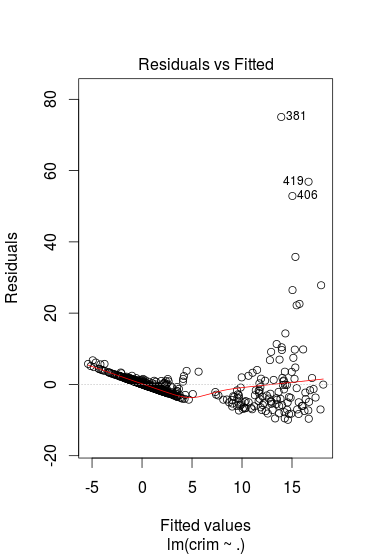
\includegraphics[scale=.60]{crimvsall.png}
\caption{Regresión crim rm}
\label{}
\end{figure}

\item Describir los resultados

EL modelo en valores entre -5 y 5 se ajusta muy bien a los datos y a partir de 5 los datos tienden a dispersarse. Esto nos muestra como los residuos del modelo de regresión múltiple tienden a tener unos valores muy similares debido a 

\item ¿Para qué predictores podemos rechazar la hipótesis nula, H0: Bj=0?

Para rechazar la hipotesis nos fijamos en Pr(>|t|) para de esta forma, si este valor estadistico es cercano a 0 podemos rechazarla.

En este caso, rechazamos la hipoteis nula para los predictores dis, rad y medv

\end{itemize}
\newpage
\subsubsection{Comparación de los resultados encontrados en los dos puntos anteriores}

\begin{itemize}

\item Crear un dibujo gráfico 2D donde cada punto del gráfico representa en el eje-X el valor de los coeficientes calculados en la regresión univariante para cada predictor y el eje-Y el valor calculado por la regresión múltiple para ese mismo predictor . Comentar el gráfico.

\begin{figure}[H]
\centering
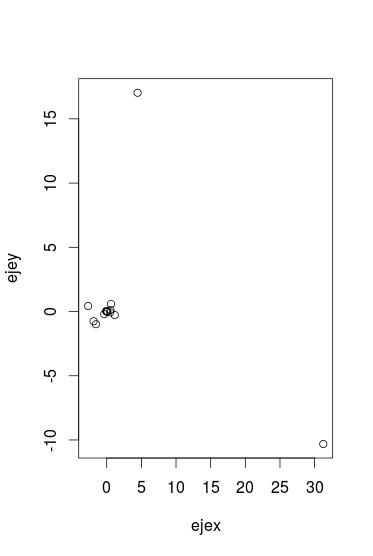
\includegraphics[scale=.60]{ejeXY.png}
\caption{Gráfico 2D coeficietes univariantes vs regresión múltiple}
\label{}
\end{figure}

Vemos como en la mayoría de predictores se obtienen valores que estan próximos al origen, esto quiere decir que los valores tanto para la regresión univariante como para la múltiple son 0. Debido  esto podemos estimar como la forma en la que se relacionan los datos frente al predictor crim son ``estables'' en cuanto a que no se observa una tendencia a crecer o decrecer, lo que si ocurre con los dos datos que están lejanos al 0. 

Esta gráfica nos es útil para ver el comportamiento general de los predictores frente a la variable crim.

\end{itemize}

\subsubsection{¿Existe evidencia de asociación no-lineal entre los predictores y la respuesta?}
\begin{itemize}

\item Apoyar la contestación ajustando un modelo lineal cúbico para cada variable predictor (Y = B0 + B1 X + B2 X 2 + B3 X 3 + e. Comentar los resultados

No existe evidencia no-lineal entre predictores y respuesta dado que, para cada predictor y ajustando un modelo de regresión cúbico, el coeficiente de correlación de pearson R-cuadrado es muy pequeño, lo que nos indica que nuestro modelo no explica lo suficiente el problema.

\end{itemize}


%----------------------------------------------------------------------------------------
%	Cuestion 3
%----------------------------------------------------------------------------------------

\subsection{Usar la base de datos “Auto data set”. Leer la base de datos.}

\subsubsection{Realizar una representación gráfica matricial (“scatterplot”) que incluya todas las representaciones de cada dos variables del conjunto de datos. Comentar lo que considere que dicha representación nos aporta en la relación entre variables.}

Observando la representación de las gráficas y fijandonos en si los valores representados en ellas obedecen a algún tipo de tendencia podemos ver como, por ejemplo, las variables mpg y displacement, horsepower y weight tienen algún tipo de relación, algo que es de esperar. También están realcionadas entre si displacement y hosrepower, hoersepower. El resto de relaciones entre variables no se podría decir a priori demasiado.

\subsubsection{Calcular la matriz de correlaciones entre variables cuantitativas usando la función cor(). Comentar los valores respecto de las gráficas del punto anterior.}

Para estas variables la matriz el valor del coeficiente de correlación alcanza valores cercanos a 1 o a -1, lo cual ratifica lo expuesto en la cuestión anterior, dado que a mayor coeficiente de correlación mas relación hay entre las variables.

\subsubsection{Usar la función lm() para realizar una regresión lineal múltiple usando “mpg” como la respuesta y todas la demás variables, excepto “name”, como predictores. Usar summary( ) para imprimir los resultados. Comentar los siguientes aspectos del resultado justificando la respuesta.}

\begin{itemize}

\item ¿Existe alguna relación entre los predictores y la respuesta?

Si, dado que el valor de R-squared es 0.8088, lo que indica que estamos explicando un alto porcentaje del modelo con estos predictores y a demás para dos de ellos (year y weight) el p-valor es igual que Pr(>|t|), lo que nos indica que el error que cometemos al elegir esos predictores es pequeño.

\item ¿Qué predictores parece tener una relación estadísticamente significativa con la respuesta?



\item ¿Que sugiere el coeficiente para la variable “year”?

Como el coeficiente de estimación es grande (0.754115) podemos decir que hay una dependencia grande entre el año y el consumo.

\end{itemize}

\subsubsection{Usando el modelo ajustado para obtener los intervalos de confianza al 95\% para los coeficientes.}

\subsubsection{Usar la función plot() para realizar dibujos de diagnóstico sobre la regresión lineal. Comentar cualquier problema que observe en el ajuste.}

\begin{figure}[H]
\centering
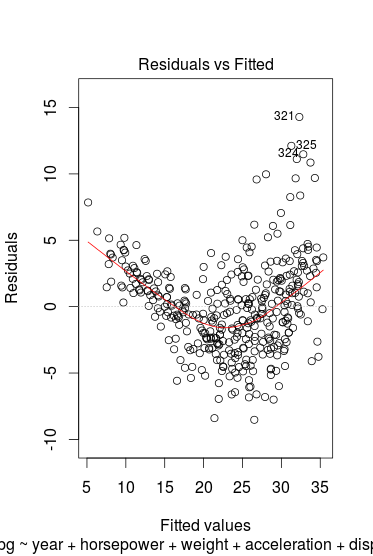
\includegraphics[scale=.60]{regmulej3.png}
\caption{Diagnóstico sobre la regresión lineal}
\label{}
\end{figure}

\begin{itemize}

\item ¿Se observan valores “outliers “ en los residuos?

Se podría hablar de una zona situada entre los valores 10 y 15 del eje Y que hacen que la recta crezca de forma que no se ajusta tanto al modelo, pero estos valores no están lo suficientemente despegados del resto de datos como para que distorsionen el modelo.

\item ¿Considera que hay algún punto con inusual alta influencia sobre el ajuste?

Si, si nos fijamos, el punto marcado como 321 parece que se despega demasiado del resto de datos e influye sobre el auste.

\end{itemize}


\subsubsection{Usar los símbolos “*” y “:” de R para ajustar un modelo de regresión lineal con términos de interacción}

\begin{itemize}

\item ¿Hay alguna interacción que sea estadísticamente significativa?

\end{itemize}

Para saber si hay alguna interacción estadisticamente significativa nos fijaremos en el p-valor y en el coeficiente de estimación.

Con esto, sería interesante incluir una interacción entre weight y horsepower, dado que su coeficiente de estimación es alto y no cometemos mucho error al introducirla. 

\end{document}